\documentclass{article}
\usepackage{PRIMEarxiv}
\usepackage[utf8]{inputenc}
\usepackage[T1]{fontenc}
\usepackage{hyperref}
\usepackage{url}
\usepackage{geometry}
\usepackage{array}
\usepackage{mathtools}
\usepackage{booktabs}
\usepackage{amsfonts}
\usepackage{amsmath}
\usepackage{amssymb}
\usepackage{nicefrac}
\usepackage{microtype}
\usepackage{lipsum}
\usepackage{fancyhdr}
\usepackage{graphicx}
\graphicspath{{media/}}
\usepackage{natbib}
\usepackage{mhchem}
\usepackage{xcolor}
\usepackage{hyperref}
\usepackage{graphicx}
\usepackage{float}
\hypersetup{
    colorlinks=true,
    linkcolor=blue,
    urlcolor=blue
}

\pagestyle{fancy}
\thispagestyle{empty}
\rhead{ \textit{ }} 

\title{ML-Guided Prediction of Movie Performance Using Movie Metadata and Sentiment Analysis}

\author{
  Jicheol Ha \\
   \\
  Columbia University \\
  New York, New York\\
  \texttt{jh4762@columbia.edu}
    \And
  Melody Huang \\
   \\
  Columbia University \\
  New York, New York \\
  \texttt{yh3802@columbia.edu} \\
    \And
  Seana Flood \\
   \\
  Columbia University \\
  New York, New York \\
  \texttt{sf3266@columbia.edu} \\
}

\usepackage{sectsty}
\sectionfont{\fontsize{16}{16}\selectfont}
\subsectionfont{\fontsize{14}{14}\selectfont}
\subsubsectionfont{\fontsize{12}{12}\selectfont}

\begin{document}
\maketitle
\vspace{-0.5cm}
\begin{abstract}
We predict gross box office revenue of American movies released after 1970 using textual and quantitative data extracted from Internet Movie Database and Rotten Tomatoes. We leverage different machine learning models and sentiment analysis to analyze how film performance is related to different movie metrics, such as popularity score, runtime,  and sentiment of audience \& critic review. Results suggest that ensemble models such as random forest and gradient boosting have higher coefficients of determination and lower mean squared error, but neural network and OLS regression minimize residual variance. Critics and audiences differ in sentiment across genres and ratings. A simple Latent Semantic Indexing model is built to recommend movies based on summary similarities. 
\end{abstract}


\section*{Introduction}
In the movie industry, accurately predicting film performance and audience reception is crucial for optimizing marketing strategies and maximizing financial returns. In this project, we predict the gross box office revenue of movies based on their attributes such as runtime, seasonality, popularity scores, obscenity ratings, and early sentiment. We first scrape data from the Internet Movie Database (IMDb) and Rotten Tomatoes, collecting information on box office earnings, plot summaries, ratings, genres, critic \& audience reviews, and other features. Using sentiment analysis, we then measure positive and negative reactions from critics and audiences, and then explore how these patterns vary across different ratings and genres. Finally, we build a recommendation system using plot similarity through a Latent Semantic Indexing (LSI) model to suggest older movies based on newer hits.

\section{Methods}
\subsection{Data Scraping}
The data was collected from two distinct sources: IMDb and Rotten Tomatoes. These platforms were chosen because while both are centered around movies, they offer different, yet complementary types of information. IMDb primarily provides objective, quantitative metrics related to a film’s performance, such as box office revenue and ratings. In contrast, Rotten Tomatoes emphasizes audience and critic perception through aggregated reviews and scores. For both data sources, web scraping was performed using Selenium in combination with Beautiful Soup to navigate dynamic content and extract the necessary information.

From IMDb, a list of 9,808 movies was compiled, restricted to English-language, color films released after January 1, 1970, with at least 3,000 user ratings. This list served two purposes: it provided the basis for feature extraction for predictive modeling, and it identified the set of movies to be scraped from Rotten Tomatoes. During this initial step, the movie title, runtime, IMDb rating, and IMDb ID were collected. For the predictive models, additional features gathered from IMDb included the IMDb rating, number of votes, number of user reviews, release date, budget, and gross box office revenue. A one-sentence summary was also collected for a subset of the movies to be used later in a Latent Semantic Indexing (LSI) analysis. From Rotten Tomatoes, both critic and audience reviews were collected. Due to the time-intensive nature of the scraping process, only a subset of the IMDb-derived movie list was used, with 40 reviews of each type gathered per selected movie.

\subsection{Data Processing}
We performed necessary data cleaning and formatting prior to predictive analysis. We removed time symbols such as `h' and `m' from runtime and computed the total number of minutes. We removed the `\$' symbol from US/Can \& Worldwide box office revenue and summed it to obtain the gross box office revenue in million USD. Popularity metrics, including  review count, star rating, and vote count, were converted to numerical values by reformatting count symbols such as `K' and `M' into integers. To capture seasonality, we extracted the month from the release date of each movie and categorized it into appropriate seasons. These were then converted to binary indicators for \texttt{spring, summer, fall,} and \texttt{winter}. Similarly, Motion Picture Association (MPA) ratings were consolidated into five categories - \texttt{G, PG, PG\_13, R}, and \texttt{Unrated} - and then converted to binary indicators. Finally, we removed entries with any null data, which resulted in a data size of $n=6772$. In Table \ref{tab:var_desc}, we describe each variable used in the predictive models.

\begin{table}[ht]
    \centering
    \caption{Variable Description}
    \begin{tabular}{l>{\raggedright}p{7cm}l}
        \toprule
        \textbf{Variable} & \textbf{Description} & \textbf{Type} \\
        \midrule
        \texttt{gross\_revenue} & Combined box office revenue from US/Canada and worldwide in million USD & Dependent \\
        \texttt{runtime} & Duration of the movie in minutes & Independent \\
        \texttt{review\_count} & Number of user reviews submitted on IMDb & Independent \\
        \texttt{star\_rating} & Average user rating on IMDb (0-10 scale) & Independent \\
        \texttt{vote\_count} & Number of votes the movie received on IMDb & Independent \\
        \texttt{spring} & Indicator for a spring release & Independent \\
        \texttt{summer} & Indicator for a summer release & Independent \\
        \texttt{fall} & Indicator for a fall release & Independent \\
        \texttt{G} & Indicator for G rating & Independent \\
        \texttt{PG} & Indicator for PG rating & Independent \\
        \texttt{PG\_13} & Indicator for PG-13 rating & Independent \\
        \texttt{R} & Indicator for R rating & Independent \\
        \bottomrule
    \end{tabular}
    \label{tab:var_desc}
\end{table}

\subsection{Multicollinearity and Heteroskedasticity}
The Variance Inflation Factor test suggests that there is minimal correlation between the independent variables, with test statistics of each variable ranging between $1$ and $8$. Thus, we retain every independent variable from Table \ref{tab:var_desc}. However, the Breusch-Pagan test statistic is $1608.04$ with a $p$-value of $0.0$, which suggests that the data is highly heteroskedastic. This negatively impacts model performance, as none of the models are able to adequately capture the nonlinearities in the data from the given attributes. Pilot residual plots of each model are characterized by a distinctive wedge-shaped distribution of residuals about zero, which confirms the presence of heteroskedasticity. In order to address this, we retain only the middle eighty percent of the data ($n=5416$) and apply the natural logarithm to the dependent variable. The Breusch-Pagan test statistic of the adjusted data is $736.18$ with a $p$-value of $9.41\cdot 10^{-151}$, which suggests that the data is still highly heteroskedastic, but there is improvement. We observe ensuing resulting improvement in model performance through another set of residual plots. 

\section{Predictive Analysis}
We ran several machine learning models to predict the gross revenue of movies from their attributes. The predictive models used in this work are ordinary least squares (OLS) regression, random forest, decision tree, gradient boosting, neural network, and light gradient boosting. We use the coefficient of determination (R-squared) and the mean squared error (MSE) between the actual and predicted box office values to evaluate model performance. We also produce residual plots to visualize model performance.

\subsection{Ordinary Least Square Regression}
To gain an insight into which factors influence gross box office revenue, we run a pilot OLS regression on the adjusted data ($n=5416$). We omit base indicator variables (\texttt{Unrated} and \texttt{winter}) from the regression. The coefficient of determination of this regression is $0.279$, which suggests that only 27.9\% of the variability in the gross revenue can be explained by the model's independent variables. The estimated OLS regression equation for predicting gross box office revenue is given by:

\begin{align*}
\log{(\texttt{gross\_revenue})} = & \, 0.1085 + 0.0157 \times \texttt{runtime} + 0.0005 \times \texttt{review\_count} \\
& - 0.1182 \times \texttt{star\_rating} + 4.103 \times 10^{-6} \times \texttt{vote\_count} \\
& - 0.2294 \times \texttt{spring} - 0.0716 \times \texttt{summer} \\
& - 0.2898 \times \texttt{fall} + 3.0811 \times \texttt{G} \\
& + 2.5980 \times \texttt{PG} + 2.3873 \times \texttt{PG-13} \\
& + 1.6946 \times \texttt{R} + \epsilon
\end{align*}

where $\epsilon$ represents the error term. In Table \ref{tab:ols_results}, we summarize the coefficients, standard errors, $t$-statistics, $p$-values, confidence intervals, and significance levels for each variable in the OLS regression. Notably, \texttt{summer} is statistically insignificant. Also, lower MPA ratings are correlated with higher percentage increases in gross box office revenue. This intuitively makes sense as movies with lower MPA ratings are available to bigger audiences. 


\begin{table}[ht]
    \centering
    \caption{Ordinary Least Squares Regression Coefficients}
    \scriptsize
    \begin{tabular}{lcccccc}
        \toprule
        \textbf{Variable} & \textbf{Coefficient} & \textbf{Std Error} & \textbf{$t$-Statistic} & \textbf{$p$-Value} & \textbf{[$0.025, 0.975$]} & \textbf{Significance} \\
        \midrule
        \texttt{runtime} & $0.0157$ & $0.001$ & $12.727$ & $<0.001$ & [$0.013, 0.018$] & *** \\
        \texttt{review\_count} & $0.0005$ & $0.000$ & $6.436$ & $<0.001$ & [$0.000, 0.001$] & *** \\
        \texttt{star\_rating} & $-0.1182$ & $0.016$ & $-7.450$ & $<0.001$ & [$-0.149$, $-0.087$] & *** \\
        \texttt{vote\_count} & $4.103\cdot 10^{-6}$ & $2.34\cdot19^{-7}$ & $17.559$ & $<0.001$ & [$3.65\cdot10^{-6}, 4.56\cdot 10^{-6}$] & *** \\
        \texttt{spring} & $-0.2294$ & $0.054$ & $-4.259$ & $<0.001$ & [$-0.335$, $-0.124$] & *** \\
        \texttt{summer} & $-0.0716$ & $0.054$ & $-1.338$ & $0.181$ & [$-0.176$, $0.033$] & - \\
        \texttt{fall} & $-0.2898$ & $0.053$ & $-5.516$ & $<0.001$ & [$-0.393$, $-0.187$] & *** \\
        \texttt{G} & $3.0811$ & $0.200$ & $15.387$ & $<0.001$ & [$2.689, 3.474$] & *** \\
        \texttt{PG} & $2.5980$ & $0.156$ & $16.633$ & $<0.001$ & [$2.292, 2.904$] & *** \\
        \texttt{PG\_13} & $2.3873$ & $0.154$ & $15.544$ & $<0.001$ & [$2.086, 2.688$] & *** \\
        \texttt{R} & $1.6946$ & $0.152$ & $11.148$ & $<0.001$ & [$1.397, 1.993$] & *** \\
        \bottomrule
        
        \textit{Note: Significance levels: ***} $p<0.001$
    \end{tabular}
    \label{tab:ols_results}
\end{table}

\subsection{Model Results and Evaluation}
We use a test-to-train ratio of $0.5$ and analyze the predictive powers of six different machine learning models. In Table \ref{tab:model_results}, we list the R-squared and MSE between actual and predicted values for each model. The metrics indicate that ensemble models such as random forest and gradient boosting outperform OLS and neural network. However, interpreting model performance solely based on these two metrics may be misleading because 1) all models are non-deterministic except for OLS and 2) the data is highly heteroskedastic. In order to address these limitations, we generate residual plots for each model (see Figure \ref{fig:residuals}). We observe a distinct wedge-shaped distribution of residuals from all models but the neural network and OLS. The residuals of these two models are approximately evenly distributed about zero, which suggests that those models are able to detect the nonlinearities in the data despite having suboptimal R-squared and MSE.

\begin{figure}[H]
    \centering
    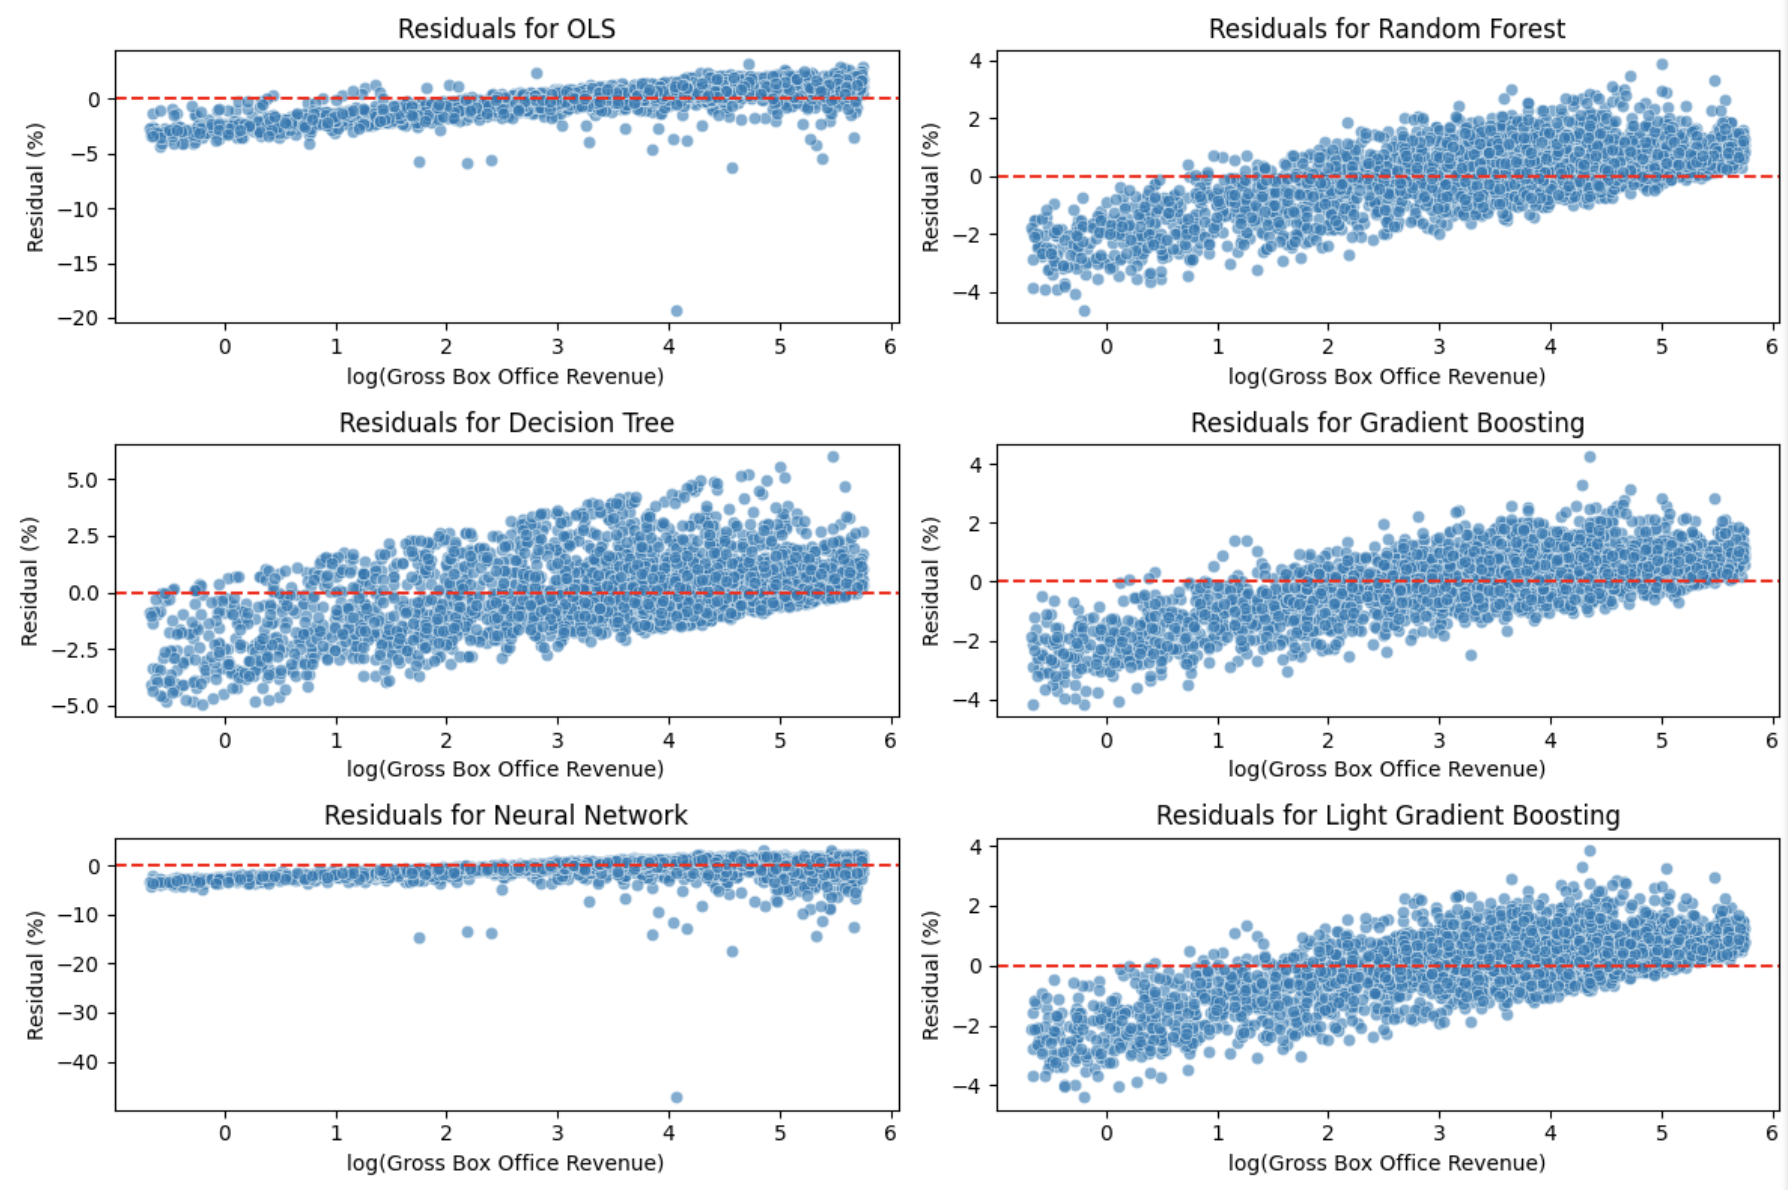
\includegraphics[width=1\textwidth]{Residuals.png}
    \caption{Residual Plots for All Models}
    \label{fig:residuals}
\end{figure} 

\begin{table}[H]
    \centering
    \caption{Coefficients of Determination and Mean Squared Error for all Models}
    \begin{tabular}{lcc}
        \toprule
        \textbf{Model Type} & \textbf{R-squared} & \textbf{Mean Squared Error} \\
        \midrule
        OLS Regression & $0.235$ & $1.97$ \\
        Random Forest $(\mathbf{n}=100)$ & $0.475$ & $1.35$ \\
        Decision Tree  & $-0.003$ & $2.58$ \\
        Gradient Boosting $(\mathbf{n}=100)$ & $0.510$ & $1.26$ \\
        Neural Network $(\mathbf{n}=[100,1], \mathbf{T_{max}}=1000)$ & $-0.597$ & $4.10$ \\
        Light Gradient Boosting $(\mathbf{n}=50)$ & $0.497$ & $1.29$ \\
        \bottomrule
    \end{tabular}
    \label{tab:model_results}
\end{table}


\section{Sentiment Analysis}
\subsection{Data Collection}
We collect movie reviews from Rotten Tomatoes for the top $10$\% highest-grossing movies ($243$ movies) identified from IMDb data. For each movie, we scrape $40$ reviews from professional critics and $40$ from general audience members. Scraping requires special handling due to Rotten Tomatoes' use of Shadow-root DOM elements, so we utilize Selenium instead of simpler methods like BeautifulSoup.

\subsection{Analyzing Sentiment}
Using sentiment analysis techniques, we calculate positive and negative sentiment percentages for each group (critics and audiences). In Table \ref{tab:sentiment_percentage}, we outline each movie’s sentiment scores, allowing easy comparison between critics' and audiences' reactions.

\begin{table}[ht]
    \centering
    \caption{Sentiment Percentage for Both Groups}
    \scriptsize
    \begin{tabular}{lcccccc}
        \toprule
        \textbf{Movie} & \textbf{Critics Positive} & \textbf{Critics Negative} & \textbf{Audience Positive} & \textbf{Audience Negative} & \textbf{Pos Diff} & \textbf{Neg Diff} \\
        \midrule
        Conspiracy Theory & $5.740741$ & $2.592593$ & $4.030091$ & $2.579258$ & $1.710649$ & $0.013334$ \\
        Christopher Robin & $6.998940$ & $1.060445$ & $4.318937$ & $1.281443$ & $2.680003$ & $-0.220997$ \\
        Five Nights at Freddy's & $3.459916$ & $3.713080$ & $3.125000$ & $1.916667$ & $0.334916$ & $1.796414$ \\
        Space Jam: A New Legacy & $4.012346$ & $2.366255$ & $4.340749$ & $2.495931$ & $-0.328403$ & $-0.129675$ \\
        The Marvels & $5.147760$ & $2.001907$ & $4.110106$ & $1.621418$ & $1.037654$ & $0.380489$ \\
        A Quiet Place Part II & $4.805077$ & $2.175884$ & $5.108557$ & $2.745849$ & $-0.303480$ & $-0.569965$ \\
        Safe Haven & $5.602923$ & $2.923264$ & $5.318040$ & $1.494612$ & $0.284884$ & $1.428652$ \\
        Alita Battle Angel & $4.771574$ & $2.030457$ & $4.254302$ & $0.956023$ & $0.517272$ & $1.074434$ \\
        Dune Part Two & $5.036630$ & $2.380952$ & $4.456654$ & $1.892552$ & $0.579976$ & $0.488400$ \\
        The Upside & $4.406130$ & $2.298851$ & $3.513283$ & $1.654135$ & $-0.907153$ & $0.644715$ \\
        \bottomrule
    \end{tabular}
    \label{tab:sentiment_percentage}
\end{table}

\subsection{Comparing Critic and Audience Sentiments}
We compare sentiment by calculating the difference in positive and negative review percentages between critics and audiences. In Figure \ref{fig:sentiment_comparison}, two scatter plots show each movie’s sentiment, with agreement along the diagonal. Critics display more extreme opinions—stronger praise or criticism—while audiences are generally more moderate. This suggests critics react more strongly, while audiences are more balanced.

\begin{figure}[H]
    \centering
    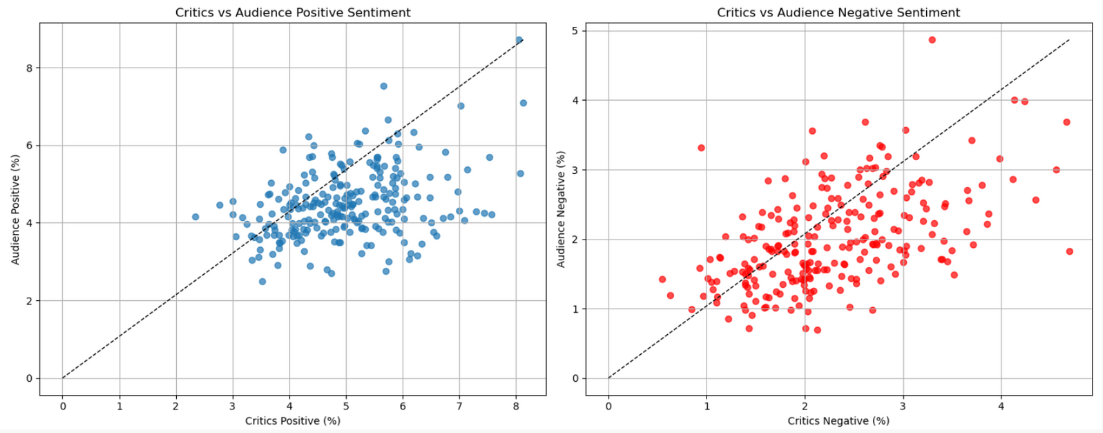
\includegraphics[width=0.8\textwidth]{ReviewScatter.png}
    \caption{Comparison of Sentiments Between Two Groups}
    \label{fig:sentiment_comparison}
\end{figure}

\subsection{Effects of Genre and Rating on Sentiment}
To dig deeper into what influences sentiment, we explore how movie MPA rating (G, PG, PG-13, R) and genre affect how people feel about films. For genres, we notice that many movies belong to multiple categories. To analyze them fairly, we “explode” the genre column—splitting each movie’s genres into separate rows—so we can evaluate each genre individually. We then calculate average sentiment scores across genres and find several clear trends: Musicals, Westerns, and Family/Kids movies consistently receive higher positive sentiment from both critics and audiences. War, Horror, and Crime genres tend to draw more negative sentiment, especially from critics (see Figure \ref{fig:sentiment_genre}).

\begin{figure}[H]
    \centering
    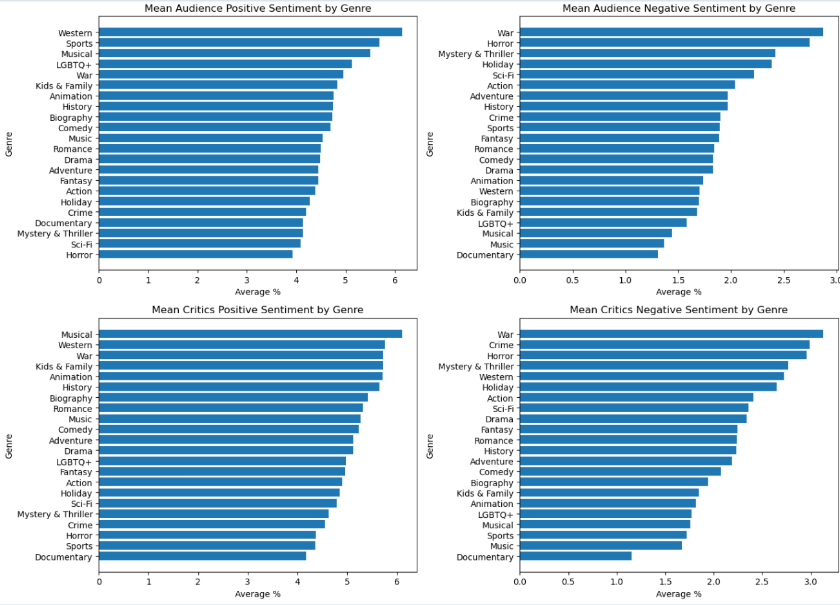
\includegraphics[width=0.95\textwidth]{Genre.png}
    \caption{Sentiment by Genre for Critics and Audiences}
    \label{fig:sentiment_genre}
\end{figure}

We observe that G and PG movies generally have higher average positive sentiment, while PG-13 and R-rated movies receive more mixed reviews. This likely reflects the fact that G/PG movies aim for broad appeal and tend to be feel-good and less polarizing, whereas R-rated films often take creative risks or explore darker content—leading to more extreme opinions (see Table \ref{tab:sentiment_by_rating}). These patterns reinforce what we see in the sentiment comparisons: lighter, family-friendly genres are more widely liked, while heavier genres and higher-rated films often divide opinion more sharply.

\begin{table}[ht]
    \centering
    \caption{Sentiment Analysis by Movie MPA Rating}
    \begin{tabular}{lcccc}
        \toprule
        \textbf{Rating} & \textbf{Positive Audience} & \textbf{Negative Audience} & \textbf{Positive Critics} & \textbf{Negative Critics} \\
        \midrule
        G & 4.618961 & 1.242318 & 6.092932 & 1.265895 \\
        PG & 4.819483 & 1.696709 & 5.646289 & 1.908592 \\
        PG-13 & 4.419307 & 2.008130 & 4.899650 & 2.305652 \\
        R & 4.258726 & 2.329682 & 4.577693 & 2.696413 \\
        \bottomrule
    \end{tabular}
    \label{tab:sentiment_by_rating}
\end{table}

\subsection{Quadrant Analysis}
To visualize how critic and audience sentiments align, we create a quadrant plot of positive sentiments (see Figure \ref{fig:quadrant_plot}). Movies are grouped into four quadrants based on median critic and audience scores:

\begin{figure}[H]
    \centering
    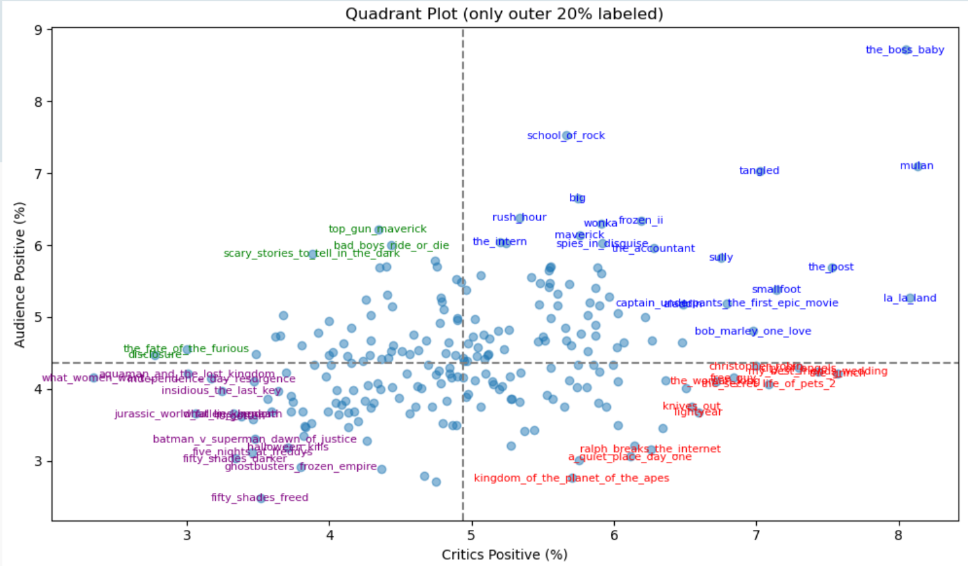
\includegraphics[width=0.9\textwidth]{QuadrantPlot.png}
    \caption{Quadrant Plot of Only Positive Sentiments}
    \label{fig:quadrant_plot}
\end{figure}

\begin{itemize}
\item Top-right: Liked by both (e.g., \textit{The Boss Baby}, \textit{La La Land}) — broad, family-friendly appeal.
\item Bottom-left: Disliked by both (e.g., \textit{Fifty Shades Freed}) — often Horror or Sci-fi.
\item Top-left: Audience favorite (e.g., \textit{Top Gun: Maverick}) — nostalgic, crowd-pleasers.
\item Bottom-right: Critic favorite (e.g., \textit{Knives Out}) — niche or complex stories.
\end{itemize}


Overall, this visualization reinforces our earlier findings, clearly showing genre and rating impacts on sentiment and highlighting key areas of agreement and disagreement between critics and audiences.

\section{Latent Semantic Indexing}
An exercise was conducted to identify the most similar movie to a given film — while not a novel concept, the intent was to explore the model’s performance using limited textual information and to satisfy general curiosity. One-sentence movie summaries from films released between 1970 and 1990 were used as the corpus, while the top 10\% of movies by box office revenue served as the reference documents. This setup aimed to identify the older film most similar to a more recent, commercially successful movie.
Various topic counts were tested to determine the optimal number for Latent Semantic Indexing, with 150 ultimately chosen. Results in the 150–300 range were largely consistent, so 150 was selected for simplicity.
However, the model's results were not particularly accurate, which was expected given the limited input. One-sentence summaries alone are insufficient to capture the depth, themes, and nuances of a movie; more comprehensive plot descriptions would likely yield better performance.

\section{Conclusion}
This project demonstrates how movie attributes and sentiment data can be used to predict box office performance. Ensemble models such as random forest and gradient boosting have higher coefficients of determination and lower mean squared error, but neural network and OLS regression demonstrate ideal residual distribution. Sentiment analysis revealed clear differences in how critics and audiences perceive films, especially across genres and rating categories. Although our Latent Semantic Indexing model had limited effectiveness due to short plot summaries, it offered a preliminary approach to content-based recommendations. Future work could enhance accuracy by incorporating richer text and optimizing model parameters.

\subsection{Limitations in Predictive Analysis}
The models were constrained by limited features and high heteroskedasticity in the data, which reduced prediction accuracy. External factors like marketing, competition, or cultural trends were not included due to data availability and scope. Good movies tend to do unpredictably well, and bad movies tend to do unpredictably badly.

\subsection{Limitations in Sentiment Analysis and Latent Semantic Indexing Models}
The sentiment analysis relied on a limited number of reviews per movie and short critic comments, which may not fully capture nuanced opinions. Additionally, using basic sentiment metrics overlooks context, sarcasm, and the depth of reviewer intent. To conserve machine runtime, we chose to use one-sentence summaries of movies rather than the multi-paragraph versions available on IMDB. While this approach limited the richness of our input data, we expect that using the longer summaries could have significantly improved our model's accuracy.
\end{document}
